\documentclass{beamer}
\usepackage{graphicx}
\usepackage{hyperref}

\usetheme[subsectionpage=progressbar]{metropolis}

\title{On Being a Research Computer Scientist}
\subtitle{or what it's like to be a lifelong learner}
\date{November 14\textsuperscript{th}, 2017}
\author{Anthony J. Christe}
\institute{University of Hawaii at Manoa \\ Slippery Rock University of Pennsylvania}

\begin{document}
\maketitle

\section{Introduction}
\begin{frame}{What People Think I Do}
\begin{figure}
	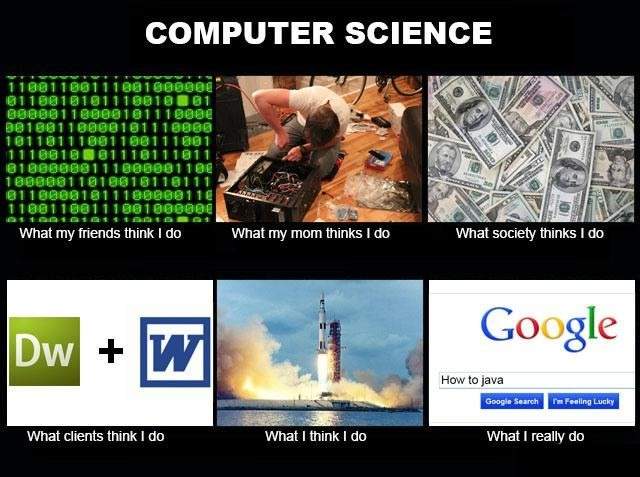
\includegraphics[width=\linewidth]{img/whatido.jpg}
\end{figure}
\end{frame}

\begin{frame}{What I actually do}
\begin{itemize}
	\item Working to obtain PhD in Computer Science
	\begin{itemize}
		\item With an emphasis on Big Data
		\item Distributed sensor networks
		\item Distributed computing
	\end{itemize}
	\item Research Assistant for Infrasound Laboratory
	\begin{itemize}
		\item Design and develop systems for capture, analysis, and reporting of infrasonic signals of interest
	\end{itemize}
\end{itemize}
\end{frame}

\begin{frame}{What Computer Science is \emph{Not}}

\end{frame}

\section{How I Got Here}
\begin{frame}{Summary of My Life Until Now}
\begin{itemize}
	\item Graduated High School
	\begin{itemize}
		\item Somerset, PA 2007
	\end{itemize}
	\item B.S. in Computer Science (w/ minor in Theatre)
	\begin{itemize}
		\item Slippery Rock University of PA, 2011
	\end{itemize}
	\item M.S. in Computer Science
	\begin{itemize}
		\item University of Hawaii at Manoa, 2015
	\end{itemize}
	\item Ph.D. in Computer Science
	\begin{itemize}
		\item University of Hawaii at Manoa, Present
	\end{itemize}
\end{itemize}
\end{frame}

\subsection{High School}
\begin{frame}{High School}
\begin{itemize}
	\item No Formal Education in Computer Science
	\item Some self taught Python
	\item Web technologies for cool AIM profiles
	\item Band Geek
	\item Theatre Geek
\end{itemize}
\end{frame}

\subsection{Undergraduate Education}
\begin{frame}{Slippery Rock University of Pennsylvania}
\begin{itemize}
	\item 
\end{itemize}
\end{frame}

\begin{frame}{Undergraduate Computer Science}
\begin{itemize}
	\item Computer Science is NOT making video games
	\item Computer Science \emph{is}
	\begin{itemize}
		\item Algorithms
		\item Data structures
		\item Software Engineering
		\item Operating Systems
		\item Artificial Intelligence
		\item Math
		\item \emph{Social}
	\end{itemize}
\end{itemize}
\end{frame}

\begin{frame}{Artificial Intelligence Robot}
\begin{itemize}
	\item Used genetic algorithms to \emph{teach} a robot to pick up a ball
	\item Machine vision and image processing were used to find the ball
	\item \url{https://www.youtube.com/watch?v=xoBVfaHHHcI}
\end{itemize}
\end{frame}

\begin{frame}{Boulders Computer Cluster}
\begin{itemize}
	\item Off the shelf parts
\end{itemize}
\end{frame}

\begin{frame}{Minor in Theatre}

\end{frame}

\begin{frame}{Other Undergrad Activities}
\begin{itemize}
	\item Vice-president of $\Upsilon\Pi$E
	\item President of Computer Technology Club
	\item Student Advisor to the Dean
\end{itemize}
\end{frame}

\subsection{Graduate School}

\begin{frame}{What is Graduate School?}
\begin{itemize}
	\item Education beyond your bachelor's degree
	\begin{itemize}
		\item Masters, Ph.D, M.D., Ed.D., \emph{etc}
	\end{itemize}
	\item Generally funded through teaching/research assistantship
	\item Specialization of your field
	\item Research focused
	\item Expects publishing and attending conferences
	\item Novel contribution to the field (Ph.D.)
\end{itemize}
\end{frame}

\begin{frame}{University of Hawaii at Manoa}
\begin{itemize}
	\item Acceptance and Making the Move
	\item Teaching Assistantship 2011-2013
	\item Master
\end{itemize}
\end{frame}

\begin{frame}{Master's Degree}

\end{frame}

\begin{frame}{Teaching Assistantship (TA)}
\begin{itemize}
	\item ICS 211 - Intro. to Programming II
	\begin{itemize}
		\item 5 Semesters
		\item Run programming lab
		\item Design homework assignments (sometimes)
		\item Grade homework assignments
		\item Run lecture (when needed)
	\end{itemize}
\end{itemize}
\end{frame}

\begin{frame}{How to get on your TA's good side?}
\begin{itemize}
	\item Show up to lab (and participate)
	\item Show up to office hours
	\item Ask questions
\end{itemize}
\end{frame}

\begin{frame}{Research Assistantship (RA)}
content...
\end{frame}

\begin{frame}{National Labs}
\begin{itemize}
	\item Lawrence Livermore National Laboratory
	\begin{itemize}
		\item Internship
		\item National Ignition Facility
	\end{itemize}
	\item Idaho National Laboratory
	\begin{itemize}
		\item Got to tour a nuclear reactor
		\item Took measurements at Yellowstone National Park
	\end{itemize}
	\item Sandia National Laboratory
\end{itemize}
\end{frame}


\begin{frame}{Conferences}
\begin{itemize}
	\item Ann Arbor, Michigan
	\item Honolulu, Hawaii
	\item Minneapolis, Minnesota
	\item San Fransisco, California
	\item Raleigh, North Carolina 
\end{itemize}
\end{frame}

\begin{frame}{Ph.D.}
\end{frame}

\section{It's Not All Hard Work}
TODO

\section{Industry}
TODO

\section{Computer Science Fields}

\begin{frame}{Computer Science Fields I}
\begin{itemize}
	\item Artificial Intelligence
	\item Computer Architecture
	\item Compiler Design
	\item Computer Graphics and Visualization
	\begin{itemize}
		\item Augmented / Visual Realty
	\end{itemize}
	\item Computer Networks
	\item Computer Security
\end{itemize}
\end{frame}

\begin{frame}{Computer Science Fields II}
\begin{itemize}
	\item Concurrency
	\item Cryptography
	\item Databases
	\item Data Science
	\item Data Structures and Algorithms
	\item Distributed Systems
	\item Formal Methods
\end{itemize}
\end{frame}

\begin{frame}{Computer Science Fields III}
\begin{itemize}

	\item High Performance Computing
	\item Human Computer Interaction (HCI)
	\item Image Processing
	\item Operating Systems
	\item Programming Languages
	\item Simulation Modeling
	\item Software Engineering
	\item Theory of Computation
\end{itemize}
\end{frame}

\begin{frame}{Thank You!}
Anthony Christe \\
achriste@hawaii.edu
\end{frame}

\end{document}
% Outline
% Title
% Meme - What people think I do
% What I actually do -- Intro only
% Outline
% How I got there -- Long store that involves robots, teaching, presenting
%	Highschool
%		What I did
% 	SRU
%		Robot
%		Theater
%		HPC - Got to present
%		Chrissie
%		What undergrad is/isn't
%		President Computer Technologu Club
%	UH
%		Masters
% 			TAing
%				Characterisitcs of kids that made it vs kids that didn't
%			OPQ
%			Infrasound, national labs, 
%		PhD		
%		It's not all work (hiking, biking, camping, take advantage of where you end up)
% That's how I got to where I am
% 
% There's also industry
%
% Computer science is a large and diverse field
% 	List of subfields and brief descriptions
% Salary information
% Shout out to UH and SRU (or maybe pick a school that specializes)
% Questions